

\section{Problem 2}
\label{part2}
\begin{verbatim}
Create an ASCII and JPEG dendrogram that clusters (i.e., HAC)
the most similar blogs (see slides 12 & 13).  Include the JPEG in
your report and upload the ascii file to github (it will be too
unwieldy for inclusion in the report).

\end{verbatim}

\subsection{Solution}
\begin{enumerate}
\item In this question I was asked to create ASCII and JPEG Dendograms that clusters the most similar blogs. 
\item In order to do this I used ``clusters.py'' code from Programming Collective Intelligence text. This code can be found in the listing\ref{lst:q2-1}.
\item I imported this code into my python file and wrote small code for generating the ASCII and Dendograms. I wrote the code by referencing to the lecture slides.
\item This code can be seen in listing\ref{lst:q2-2}.
\item Dendogram file can be seen in the fig\ref{Samplet1} and ASCII file can be seen in the fig\ref{Samplet2}.
\item Unfortunately, Dendogram is difficult to see, but from this Dendogram we can infer that the blogs similar to ``F-Measure'' is ``Samtastic! Review'' and the blog similar to ``'Web Science and Digital Library Research Group '' is ``Mile In Mine''.
\end{enumerate}
\newpage

\subsection{Code Listing}

\lstinputlisting[language=Python,breaklines = true,frame=single,caption={Python Code for clustering from PCI text}, label=lst:q2-1,captionpos=b,numbers=left,showspaces=false,showstringspaces=false,basicstyle=\footnotesize]{clusters.py}
\newpage

\subsection{Code Listing}

\lstinputlisting[language=Python,breaklines = true,frame=single,caption={Python Code for getting ASCII and JPEG dendogram}, label=lst:q2-2,captionpos=b,numbers=left,showspaces=false,showstringspaces=false,basicstyle=\footnotesize]{q2.py}
\newpage

\subsection{Outputs}
\subsubsection{Dendogram}
\begin{figure}[ht]    
    \begin{center}
        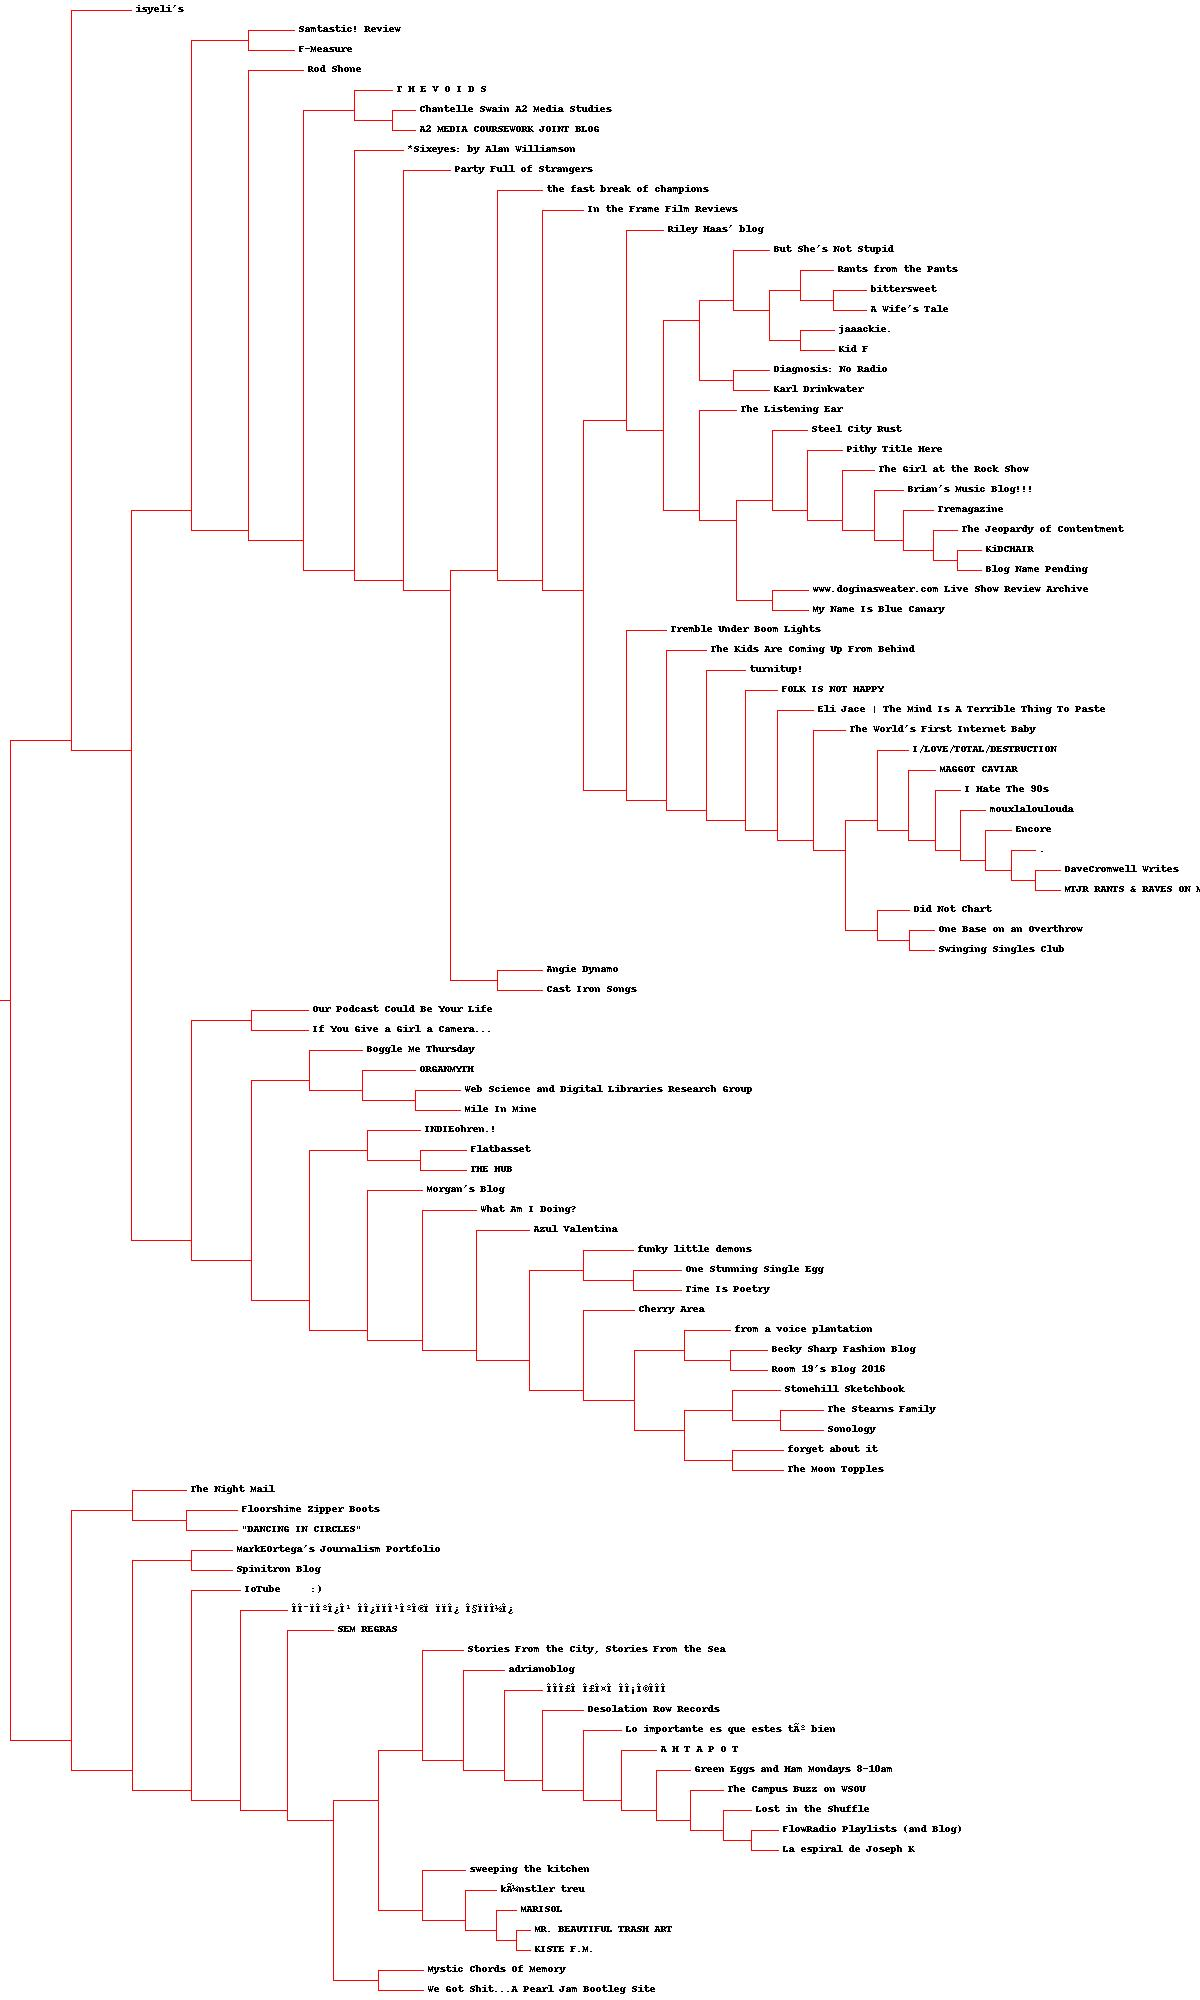
\includegraphics[scale=0.24]{clusterblog.jpg}
        \caption{Dendogram clustering most similar blogs}
        \label{Samplet1}
    \end{center}
\end{figure}
\newpage

\subsubsection{ASCII file}
\begin{figure}[ht]    
    \begin{center}
        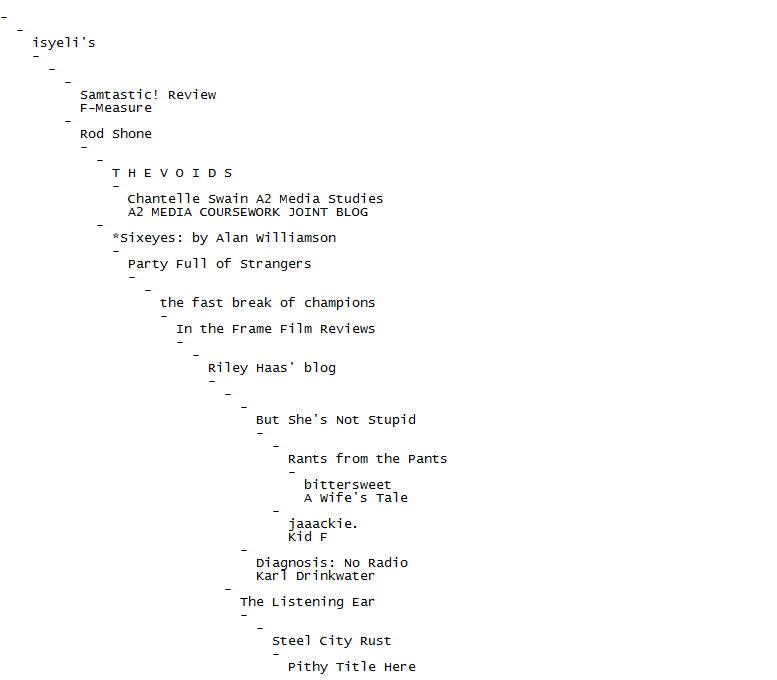
\includegraphics[scale=0.8]{sample_ascii_2.png}
        \caption{ASCII file showing clustering of most similar blogs}
        \label{Samplet2}
    \end{center}
\end{figure}
\newpage
